\documentclass[12pt]{beamer}
\usepackage[utf8]{inputenc}
%\usepackage[latin1]{inputenc}
\usepackage[spanish]{babel}
%\usetheme{Warsaw}
%\usepackage{euler}
\usepackage{amsmath}
\usepackage{amsthm}
\usepackage{multicol}
\usepackage{multirow}
\usepackage{graphicx}
\usepackage{tikz}
\usepackage{color}
\usepackage{listings}

\include{pream_codigo}
\DeclareGraphicsExtensions{.pdf,.png,.jpg}
\renewcommand {\arraystretch}{1.5}
\mode<presentation>
{
  \usetheme{Warsaw}
  \setbeamercovered{transparent}
  % or whatever (possibly just delete it)
}
\title{Tema 1 - Soluci\'{o}n del examen}
\subtitle{Curso de F\'{i}sica Computacional}
\author{M. en C. Gustavo Contreras May\'{e}n}
%\email{curso.fisica.comp@gmail.com}
%\ptsize{10}
\begin{document}
\maketitle
\fontsize{14}{14}\selectfont
\spanishdecimal{.}
\begin{frame}{Contenido}
\tableofcontents[pausesections]
\end{frame}
\section{Problema 2}
\begin{frame}
\frametitle{Problema 2}
Un problema cl\'{a}sico en c\'{o}mputo cient\'{i}fico, es la suma de una serie para evaluar una funci\'{o}n. Sea la serie de potencias para la funci\'{o}n exponencial:
\[e^{-x} = 1 - x + \dfrac{x^{2}}{2!} - \dfrac{x^{3}}{3!} +\cdots \hspace{1.5cm} (x^{2} < \infty)  \]
Utiliza la serie anterior para calcular el valor de $e^{-x}$ para $x=0.1,1,10, 100, 1000$ con un error absoluto para cada caso, menor a $10^{-8}$
\end{frame}
\begin{frame}
Tomemos en cuenta que no est\'{a} indicado el punto en donde se debe de cortar la serie de potencias, por lo que nuestra tarea es calcular el valor de $\exp(-x)$ de tal manera en que se calcule el error y se revise que sea menor a $10^{-8}$:
\begin{center}
	\begin{tabular}{l | l | l}
	x & valor & t\'{e}rmino \\ \hline
	0.1 &  &  \\ \hline
	1 &  &  \\ \hline
	10 &  &  \\ \hline
	100 &  &  \\ \hline
	1000 &  &
	\end{tabular}
\end{center}
\end{frame}
\begin{frame}
Podemos crear una funci\'{o}n que nos calcule el valor de la exponencial con el argumento y que revise el error debido entre la diferencia del valor calculado contra el valor exacto que tomamos de $\exp(x)$.
\\
\medskip
Y para hacer el proceso m\'{a}s eficiente, podemos incluir un ciclo que calcule los valores y diferencias en un s\'{o}lo paso.
\end{frame}
\begin{frame}
\frametitle{Tabla de resultados completa}
\fontsize{12}{12}\selectfont
\begin{center}
	\begin{tabular}{l | l | l | l}
	x & n & $\exp(-x)$ & valor \\ \hline 
	0.1 & 6 & 0.9048374180359595 & 0.9048374166666667 \\ \hline
	1 & 12 & 0.36787944117144233 & 0.367879439233606 \\ \hline
	10 & 40 & 4.5399929762484854e-05 & 4.539008559460963e-05 \\ \hline
	100 & & & \\ \hline
	1000 & & &
	\end{tabular}
\end{center}
Vemos que para valores de 100 y 1000, Python ya se queja por un \textbf{Overflow}.
\end{frame}
\section{Problema 3}
\begin{frame}
\frametitle{Problema 3}
Usando el m\'{e}todo de Horner, completa la tabla de valores de los puntos de evaluaci\'{o}n y el valor calculado con el m\'{e}todo de Horner; el polinomio es:
\[p(x)= 2x^{4} - 20x^{3} + 70x^{2}+ 100x+48 \]
para valores de $x$ en el intervalo $[-4,-1]$, con saltos de $x$ de valor $\Delta x = 0.5$.
\medskip
\\
Grafica los puntos obtenidos y el polinomio $p(x)$, interpreta los resultados obtenidos.
\end{frame}
\begin{frame}
Primeramente tenemos que completar la tabla:
\begin{center}
	\begin{tabular}{l | l}
	x & valor \\ \hline
	-4.0 & \\ \hline
	-3.5 & \\ \hline
	-3.0 & \\ \hline
	$\ldots$ & \\ \hline
	-1.5 & \\ \hline
	-1.0 & 
	\end{tabular}
\end{center}
\end{frame}
\begin{frame}
Usamos el c\'{o}digo que ya hab\'{i}amos discutido en una de las clase; obtenemos entonces el siguiente resultado:
\begin{center}
	\begin{tabular}{l | l}
	x & valor \\ \hline
	-4.0 & 2560.0 \\ \hline
	-3.5 & 1713.125 \\ \hline
	-3.0 & 1080.0 \\ \hline
	-2.5 & 626.125 \\ \hline
	-2.0 & 320.0 \\ \hline
	-1.5 & 133.125 \\ \hline
	-1.0 & 40.0
	\end{tabular}
\end{center}
\end{frame}
\begin{frame}
\begin{figure}
	\centering
	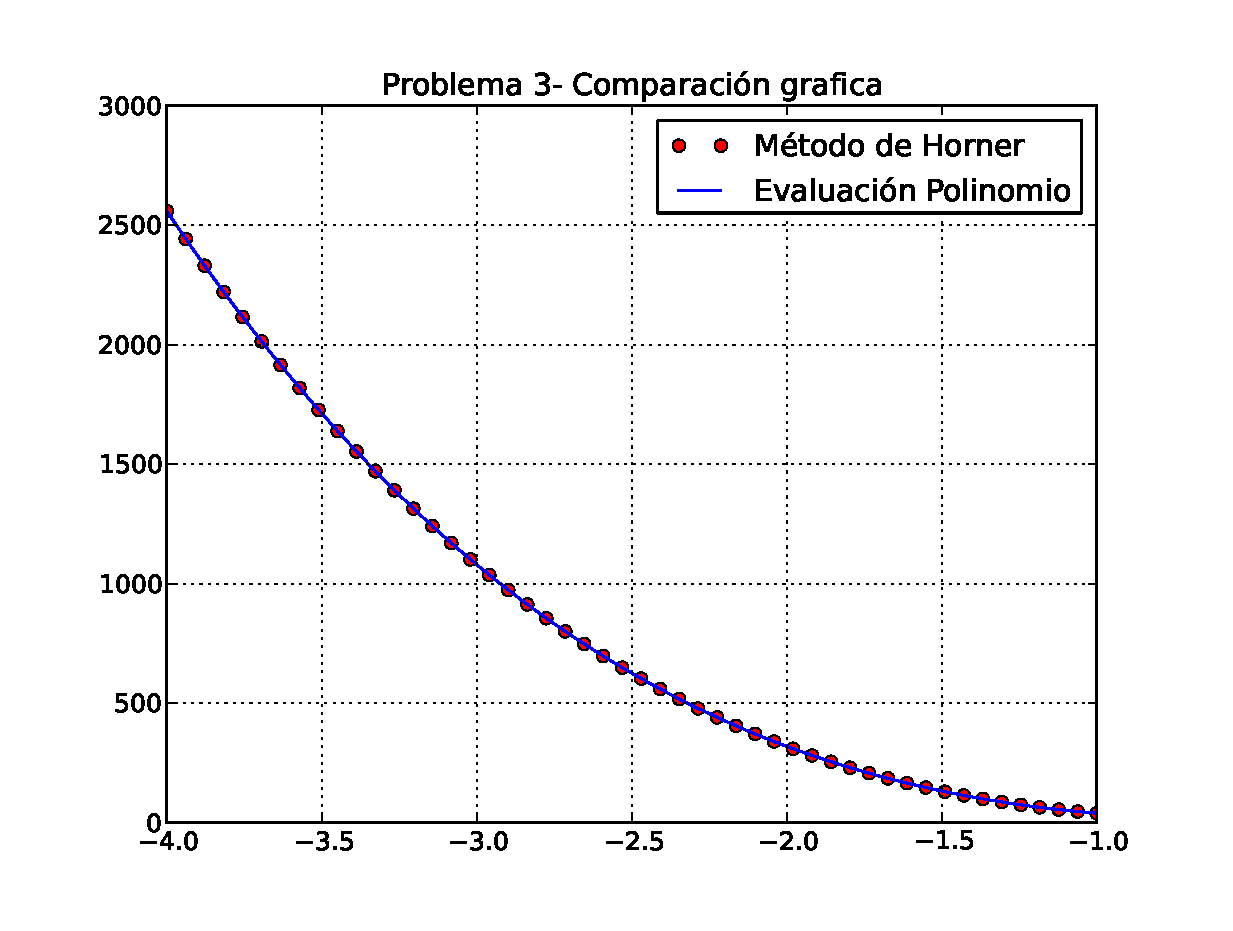
\includegraphics[scale=0.45]{E1_Problema3.eps} 
\end{figure}
\end{frame}
\section{Problema 4}
\begin{frame}
\frametitle{Problema 4}
El valor de $\pi$ se puede calcular aproximando el \'{a}rea de un c\'{i}rculo unitario como el l\'{i}mite de una sucesi\'{o}n $p_{1}, p_{2}, \ldots$ descrita a continuaci\'{o}n:
\\
Se divide un c\'{i}rculo unitario en $2^{n}$ sectores (en el ejemplo, $n=3$). Se aproxima el \'{a}rea del sector por el \'{a}rea del tri\'{a}ngulo is\'{o}celes. El \'{a}ngulo $\theta_{n}$ es $2 \pi / 2^{n}$. El \'{a}rea del tri\'{a}ngulo es $1/2 \sin \theta_{n}$.
\end{frame}
\begin{frame}
\begin{figure}[H]
\centering
\begin{tikzpicture}
\draw (3,3) circle (2);
\draw (1,3) -- (5,3);
\draw (3,1) -- (3,5);
\draw (1.6,4.39) -- (4.39,1.6);
\draw (4.39,4.39) -- (1.6,1.6);
\draw (4.39,4.39) -- (5,3);
\draw (5,3) -- (4.39,1.6);
\draw (5,3) -- (4.39,1.6);
\draw (4.39,1.6) -- (3,1);
\draw (3,1) -- (1.6,1.6);
\draw (1.6,1.6) -- (1,3);
\draw (1,3) -- (1.6,4.39);
\draw (1.6,4.39) -- (3,5);
\draw (3,5) -- (4.39,4.39);
\draw (3.3,3) arc (0:16:1);
\draw [font=\small] (3.7,3.2) node {$\theta_{n}$};
\draw [font=\small] (3.7,4) node {1};
\draw [font=\small] (4.2,2.8) node {1};
\end{tikzpicture}
\caption{Divisi\'{o}n en $n$ sectores.}
\end{figure}
\end{frame}
\begin{frame}
La en\'{e}sima aproximaci\'{o}n a $\pi$ es: $p_{n}= 2^{n-1} \sin \theta_{n}$. Demuestra que
\[\sin \theta_{n} = \dfrac{\sin \theta_{n-1}}{\left( 2 \left[ 1+ (1-\sin^{2}\theta_{n-1})^{\frac{1}{2}} \right] \right)^{\frac{1}{2}}} \]
Usa esta relaci\'{o}n de recurrencia para generar las sucesiones $\sin \theta_{n}$ y $p_{n}$ en el rango $3 \leq n \leq 20$ iniciando con $\sin \theta_{2}=1$. Compara tus resultados con el valor de $4.0 \arctan(1.0)$
\end{frame}
\begin{frame}
Para este ejercicio lo que hacemos es obtener primero el valor del $\sin(\theta_{n})$ y despu\'{e}s, ocupar ese valor para el c\'{a}lculo del valor de $p_{n}$, aqu\'{i} mismo podemos obtener el valor del error relativo, por lo que tendremos una tabla del tipo:
\end{frame}
\begin{frame}
\begin{center}
	\begin{tabular}{l | l | l}
	n & valor de $\pi$ & error \\ \hline
	3 & 2.82842712475 & 1.107207e-01 \\ \hline
	4 & 3.06146745892 & 2.617215e-02 \\ \hline
	5 & 3.12144515226 & 6.454543e-03 \\ \hline
	6 & 3.13654849055 & 1.608189e-03 \\ \hline
	7 & 3.14033115695 & 4.017082e-04 \\ \hline
	\ldots & & \\ \hline
	19 & 3.14159265351 & 2.393685e-11 \\ \hline
	20 & 3.14159265357 & 5.984108e-12 \\ \hline
	\end{tabular}
\end{center}
\end{frame}
\begin{frame}
Para comprender lo que ocurre mientras aumentamos el n\'{u}mero de segmentos y el valor del \'{a}rea, lo tenemos al graficar:
\begin{figure}
	\centering
	\includegraphics[scale=0.4]{E1_Problema4.eps} 
\end{figure}
\end{frame}
\section{Problema 5}
\begin{frame}
\frametitle{Problema 5}
La sucesi\'{o}n de Fibonacci $1,1,2,3,5,8,13,\ldots$ est\'{a} definida por la relaci\'{o}n de recurrencia lineal
\begin{equation*}
\begin{cases}
\lambda_{1} = 1 \hspace{0.5cm} \lambda_{2}= 1 \\
\lambda_{n} = \lambda_{n-1} + \lambda_{n-2} \hspace{0.5cm} (n \geq 3)
\end{cases}
\end{equation*}
\end{frame}
\begin{frame}
Una f\'{o}rmula para obtener el n-\'{e}simo n\'{u}mero de Fibonacci es
\[ \lambda_{n} = \dfrac{1}{\sqrt{5}} \left\lbrace \left[ \dfrac{1}{2} (1 + \sqrt{5}) \right]^{n} - \left[ \dfrac{1}{2} (1 - \sqrt{5}) \right]^{n} \right\rbrace \]
Calcula $\lambda_{n}$ en $3\leq n \leq 50$ usando tanto la relaci\'{o}n de recurrencia como la f\'{o}rmula. Discute los resultados obtenidos.
\end{frame}
\begin{frame}
Para resolver este problema, lo que tenemos que hacer es definir un par de funciones que nos devuelvan el valor del n-\'{e}simo n\'{u}mero de la serie de Fibonacci, para luego obtener el error relativo.
\end{frame}
\begin{frame}
La manera para presentar los resultados, ser\'{i}a en una tabla del tipo:
\fontsize{12}{12}\selectfont
\begin{center}
	\begin{tabular}{l | l | l | l}
	n & M1 & M2 & error \\ \hline
	3 & 2 & 2.000000000000000 & 0.00e+00 \\ \hline
	4 & 3 & 3.000000000000000 & 1.48e-16 \\ \hline
	5 & 5 & 5.000000000000001 & 1.78e-16 \\ \hline
	6 & 8 & 8.000000000000002 & 2.22e-16 \\ \hline
	7 & 13 & 13.000000000000002 & 1.37e-16 \\ \hline
 	$\ldots$ & & &   \\ \hline
 	48 & 4807526976 & 4807526976.000007629394531 & 1.59e-15 \\ \hline
	49 & 7778742049 & 7778742049.000013351440430 & 1.72e-15 \\ \hline
	50 & 12586269025 & 12586269025.000019073486328 & 1.52e-15
	\end{tabular}
\end{center}
\end{frame}
\begin{frame}
Para tener una idea visual del resultado, graficamos el valor de $\pi$ contra los $2^{n}$ sectores:
\begin{figure}
	\centering
	\includegraphics[scale=0.4]{E1_Problema5.eps} 
\end{figure}
\end{frame}
\end{document}